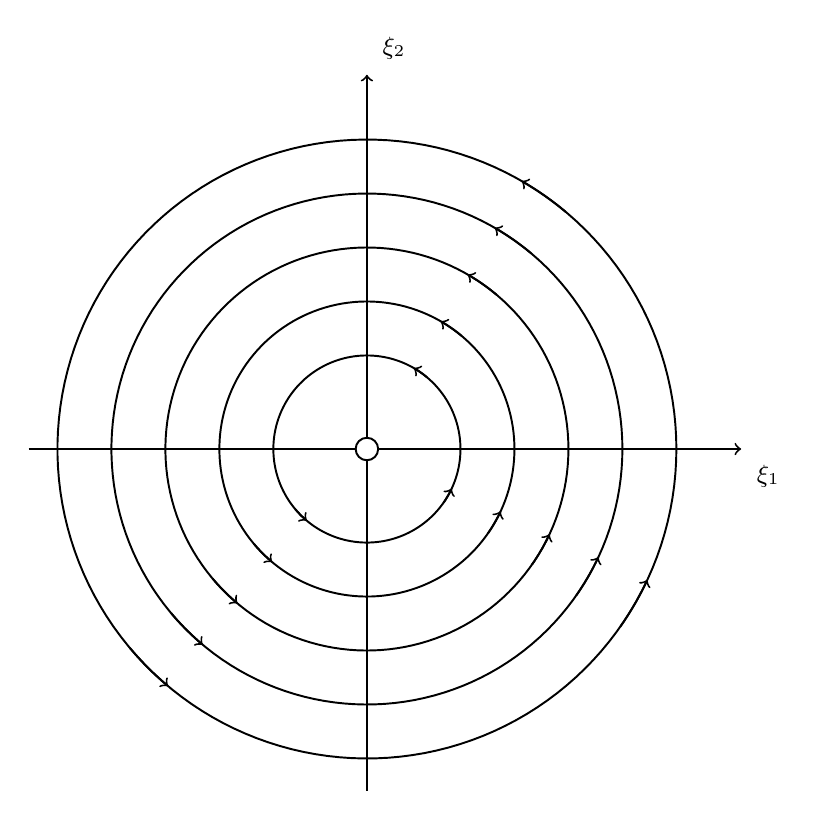
\begin{tikzpicture}[scale=2.5390,font=\small,x=0.9cm,y=0.9cm,line width=0.7pt]
  % xi_1'=-xi_2, xi_2'=xi_1: concentric counterclockwise periodic orbits.
  \foreach \r in {0.52,0.82,1.12,1.42,1.72} {
    \draw plot[domain=0:360,samples=160,variable=\a]
      ({\r*cos(\a)},{\r*sin(\a)})--cycle;
    \foreach \b in {55,225,330} {
      \draw[->] plot[domain={\b-5}:{\b+5},samples=9,variable=\a]
        ({\r*cos(\a)},{\r*sin(\a)});
    }
  }
  \draw[->] (-1.88,0)--(2.08,0);
  \draw[->] (0,-1.90)--(0,2.08);
  \fill[white] (0,0) circle (1.6pt);
  \draw (0,0) circle (1.6pt);
  \node[below right=2pt] at (2.08,0) {$\xi_1$};
  \node[above right=2pt] at (0,2.08) {$\xi_2$};
\end{tikzpicture}
